\lecture{输入输出流与文件系统}{lec:chap08}
\section[流类]{输入输出流类}\label{sec:chap08-sec01}
%%%%%%%%%%%%%%%%%%%%%%%%%%%%%%%%%%%%%%%%%%%%%%%%%%%%%%%%%%%%%%%%%%%%%%%%%%%%%%%
\begin{frame}[t, fragile]{输入输出流类}{简介}%
  \begin{itemize}
  \item 什么是流(stream)
    \begin{itemize}
    \item 与物理输入输出设备无关的数据序列
    \end{itemize}
  \end{itemize}
  \begin{center}
    \begin{tikzpicture}[font=\tiny, show background grid]
      \tikzset{ coord/.style={coordinate} }
      
      \node (fig1) at (0, 0)
      {
        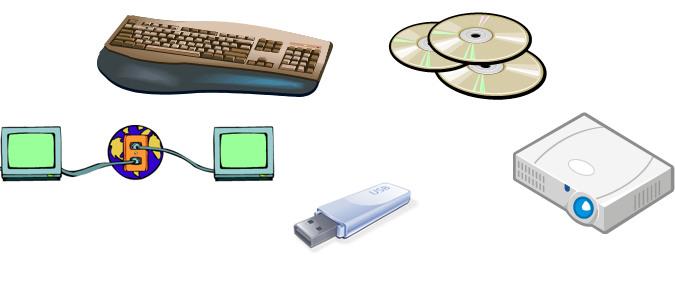
\includegraphics[width=0.4\textwidth]{figure/chap08/01inputdevice}
      };

      \node[right=1.3 of fig1] (fig2)
      {
        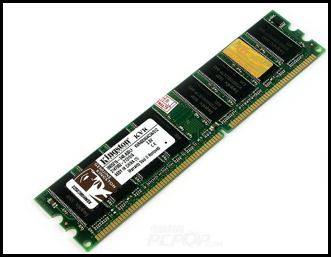
\includegraphics[width=0.3\textwidth]{figure/chap08/02mem}
      };

      \node[below=1.3 of fig2] (fig3)
      {
        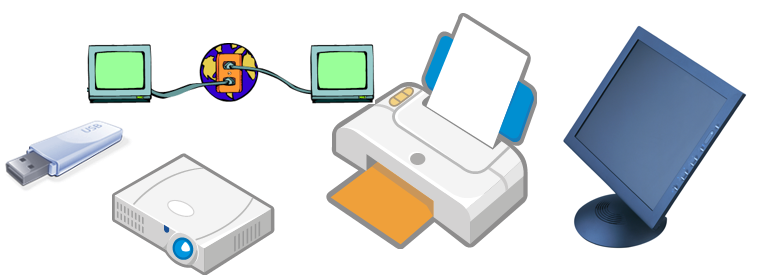
\includegraphics[width=0.4\textwidth]{figure/chap08/03outputdevice}
      };
      \draw[-{Stealth[scale=1.0]}, red, thick] (fig1.east) to [out =
      0, in = 180] (fig2.west);
      \draw[-{Stealth[scale=1.0]}, red, thick] (fig2.south) to [out =
      -90, in = 90] (fig3.north);
    \end{tikzpicture}
  \end{center}
\end{frame}

\begin{frame}[t, fragile]{输入输出流类}{类模板层次结构}%
  \begin{itemize}
  \item 输入输出流类模板层次结构图
  \end{itemize}
  \begin{center}
    \begin{tikzpicture}[font=\tiny, show background grid]
      \tikzset{ coord/.style={coordinate} }

      \begin{class}[scale=1.0, text width=0.8cm ]{ios-base} {0, 1.5}
      \end{class}

      \begin{class}[scale=1.0, text width=1.5cm] {basic-ios} {0, 0}
        \inherit{ios-base}
      \end{class}

      \begin{class}[scale=1.0, text width=1.5cm ]{basic-istream}{-2.0, -1.5}
        \inherit{basic-ios}
      \end{class}

      \begin{class}[scale=1.0, text width=1.5cm ]{basic-ostream}{2.0, -1.5}
        \inherit{basic-ios}
      \end{class}

      \begin{class}[scale=1.0, text width=1.5cm ]{basic-ifstream}{-3.0,  -3.0}
        \inherit{basic-istream}
      \end{class}

      \begin{class}[scale=0.8, text width=1.5cm ]{basic-iostream}{0.0, -3.0}
        \inherit{basic-istream}
        \inherit{basic-ostream}
      \end{class}

      \begin{class}[scale=1.0, text width=1.5cm ]{basic-ofstream}{3.0, -3.0}
        \inherit{basic-ostream}
      \end{class}

      \begin{class}[scale=1.0, text width=1.5cm ]{basic-fstream}{0.0, -4.3}
        \inherit{basic-iostream}
      \end{class}

      % \umlnote[scale=0.6,text width=1.2cm, left=of ifstream](note1)
      % {Defined in fsteam.h}; \umlnote[scale=0.6,text width=1.2cm,
      % right=of ofstream](note2) {Defined in fsteam.h};

      % \draw[red, dashed, thick](note1) -- (ifstream); \draw[red,
      % dashed, thick](note2) -- (ofstream);
    \end{tikzpicture}
  \end{center}
\end{frame}

\begin{frame}[t, fragile]{输入输出流类}{字符集}%
  \begin{itemize}
  \item 类模板可实例化为窄字符类(\cppinline{char})和宽字符类(\cppinline{wchar_t})
  \end{itemize}
  \begin{center}
    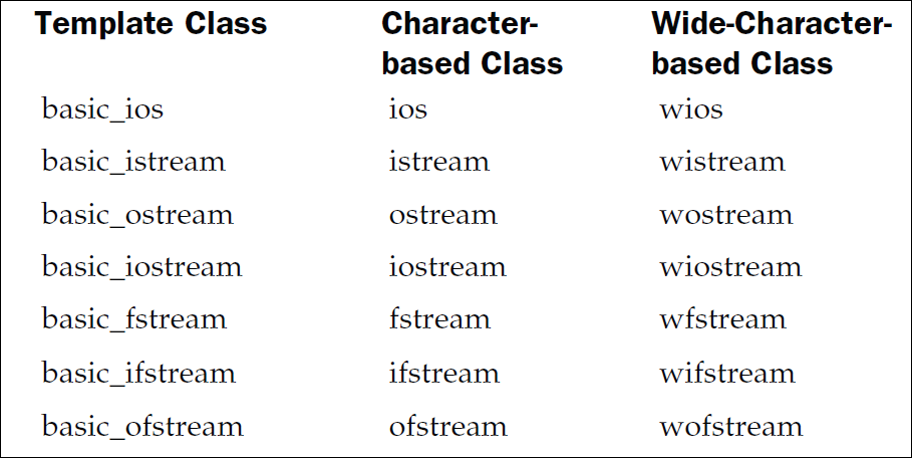
\includegraphics[width=0.95\textwidth]{figure/chap08/04charset}
  \end{center}
\end{frame}

\begin{frame}[t, fragile]{输入输出流类}{类模板层次结构}%
  \begin{itemize}
  \item 输入输出流类模板层次结构图
  \end{itemize}
  \begin{center}
    \begin{tikzpicture}[font=\tiny, show background grid]
      \tikzset{ coord/.style={coordinate} }

      \begin{class}[scale=1.0, text width=0.8cm ]{ios-base} {0, 1.5}
      \end{class}

      \begin{class}[fill=green!25, scale=1.0, text width=1.5cm] {ios} {0, 0}
        \inherit{ios-base}
      \end{class}

      \begin{class}[fill=green!25, scale=1.0, text width=1.5cm ]{istream}{-2.0, -1.5}
        \inherit{ios}
      \end{class}

      \begin{class}[fill=green!25, scale=1.0, text width=1.5cm ]{ostream}{2.0, -1.5}
        \inherit{ios}
      \end{class}

      \begin{class}[scale=1.0, text width=1.5cm ]{ifstream}{-3.0,  -3.0}
        \inherit{istream}
      \end{class}

      \begin{class}[fill=green!25, scale=0.8, text width=1.5cm ]{iostream}{0.0, -3.0}
        \inherit{istream}
        \inherit{ostream}
      \end{class}

      \begin{class}[scale=1.0, text width=1.5cm ]{ofstream}{3.0, -3.0}
        \inherit{ostream}
      \end{class}

      \begin{class}[scale=1.0, text width=1.5cm ]{fstream}{0.0, -4.3}
        \inherit{iostream}
      \end{class}

      \umlnote[scale=1.0, text width=2.5cm](note1) at (3.0, 0.5)
      {输入输出流的格式化、\\错误检测和其它状态信息};

      \draw[-{Stealth[scale=1.0]}, red, thick](ios.east) to
      [out = 0, in = 180] (note1.west); 
    \end{tikzpicture}
  \end{center}
\end{frame}

\begin{frame}[t, fragile]{输入输出流类}{类模板层次结构}%
  \begin{itemize}
  \item 输入输出流类模板层次结构图
  \end{itemize}
  \begin{center}
    \begin{tikzpicture}[font=\tiny, show background grid]
      \tikzset{ coord/.style={coordinate} }

      \begin{class}[scale=1.0, text width=0.8cm ]{ios-base} {0, 1.5}
      \end{class}

      \begin{class}[fill=green!25, scale=1.0, text width=1.5cm] {ios} {0, 0}
        \inherit{ios-base}
      \end{class}

      \begin{class}[fill=green!25, scale=1.0, text width=1.5cm ]{istream}{-2.0, -1.5}
        \inherit{ios}
      \end{class}

      \begin{class}[fill=green!25, scale=1.0, text width=1.5cm ]{ostream}{2.0, -1.5}
        \inherit{ios}
      \end{class}

      \begin{class}[scale=1.0, text width=1.5cm ]{ifstream}{-3.0,  -3.0}
        \inherit{istream}
      \end{class}

      \begin{class}[fill=green!25, scale=0.8, text width=1.5cm ]{iostream}{0.0, -3.0}
        \inherit{istream}
        \inherit{ostream}
      \end{class}

      \begin{class}[scale=1.0, text width=1.5cm ]{ofstream}{3.0, -3.0}
        \inherit{ostream}
      \end{class}

      \begin{class}[scale=1.0, text width=1.5cm ]{fstream}{0.0, -4.3}
        \inherit{iostream}
      \end{class}

      \umlnote[scale=1.0, text width=2.5cm](note1) at (-3.0, 0.5)
      {输入操作,包括\cppintttny{get}、\cppintttny{getline}、\cppintttny{read}、\cppintttny{seekg}和“\cppintttny{>>}”重载函数};

      \draw[-{Stealth[scale=1.0]}, red, thick](istream.north) to
      [out = 90, in = -90] (note1.south); 
    \end{tikzpicture}
  \end{center}
\end{frame}

\begin{frame}[t, fragile]{输入输出流类}{类模板层次结构}%
  \begin{itemize}
  \item 输入输出流类模板层次结构图
  \end{itemize}
  \begin{center}
    \begin{tikzpicture}[font=\tiny, show background grid]
      \tikzset{ coord/.style={coordinate} }

      \begin{class}[scale=1.0, text width=0.8cm ]{ios-base} {0, 1.5}
      \end{class}

      \begin{class}[fill=green!25, scale=1.0, text width=1.5cm] {ios} {0, 0}
        \inherit{ios-base}
      \end{class}

      \begin{class}[fill=green!25, scale=1.0, text width=1.5cm ]{istream}{-2.0, -1.5}
        \inherit{ios}
      \end{class}

      \begin{class}[fill=green!25, scale=1.0, text width=1.5cm ]{ostream}{2.0, -1.5}
        \inherit{ios}
      \end{class}

      \begin{class}[scale=1.0, text width=1.5cm ]{ifstream}{-3.0,  -3.0}
        \inherit{istream}
      \end{class}

      \begin{class}[fill=green!25, scale=0.8, text width=1.5cm ]{iostream}{0.0, -3.0}
        \inherit{istream}
        \inherit{ostream}
      \end{class}

      \begin{class}[scale=1.0, text width=1.5cm ]{ofstream}{3.0, -3.0}
        \inherit{ostream}
      \end{class}

      \begin{class}[scale=1.0, text width=1.5cm ]{fstream}{0.0, -4.3}
        \inherit{iostream}
      \end{class}

      \umlnote[scale=1.0, text width=2.5cm](note1) at (3.0, 0.5)
      {输出操作,包括\cppintttny{put}、\cppintttny{write}、
        \cppintttny{seekp}和“\cppintttny{<<}”重载函数};
      
      \draw[-{Stealth[scale=1.0]}, red, thick](ostream.north) to
      [out = 90, in = -90] (note1.south); 
    \end{tikzpicture}
  \end{center}
\end{frame}

\begin{frame}[t, fragile]{输入输出流类}{类模板层次结构}%
  \begin{itemize}
  \item 输入输出流类模板层次结构图
  \end{itemize}
  \begin{center}
    \begin{tikzpicture}[font=\tiny, show background grid]
      \tikzset{ coord/.style={coordinate} }

      \begin{class}[scale=1.0, text width=0.8cm ]{ios-base} {0, 1.5}
      \end{class}

      \begin{class}[fill=green!25, scale=1.0, text width=1.5cm] {ios} {0, 0}
        \inherit{ios-base}
      \end{class}

      \begin{class}[fill=green!25, scale=1.0, text width=1.5cm ]{istream}{-2.0, -1.5}
        \inherit{ios}
      \end{class}

      \begin{class}[fill=green!25, scale=1.0, text width=1.5cm ]{ostream}{2.0, -1.5}
        \inherit{ios}
      \end{class}

      \begin{class}[scale=1.0, text width=1.5cm ]{ifstream}{-3.0,  -3.0}
        \inherit{istream}
      \end{class}

      \begin{class}[fill=green!25, scale=0.8, text width=1.5cm ]{iostream}{0.0, -3.0}
        \inherit{istream}
        \inherit{ostream}
      \end{class}

      \begin{class}[scale=1.0, text width=1.5cm ]{ofstream}{3.0, -3.0}
        \inherit{ostream}
      \end{class}

      \begin{class}[scale=1.0, text width=1.5cm ]{fstream}{0.0, -4.3}
        \inherit{iostream}
      \end{class}

      \umlnote[scale=1.0, text width=2.5cm](note1) at (3.0, 0.5)
      {无新增成员,定义了\cppintttny{cin}、\cppintttny{cout}、
        \cppintttny{cerror}和“\cppintttny{clog}”对象};
      
      \draw[-{Stealth[scale=1.0]}, red, thick](iostream.north) to
      [out = 90, in = -90] (note1.south); 
    \end{tikzpicture}
  \end{center}
\end{frame}

\begin{frame}[t, fragile]{输入输出流类}{类模板层次结构}%
  \begin{itemize}
  \item 输入输出流类模板层次结构图
  \end{itemize}
  \begin{center}
    \begin{tikzpicture}[font=\tiny, show background grid]
      \tikzset{ coord/.style={coordinate} }

      \begin{class}[scale=1.0, text width=0.8cm ]{ios-base} {0, 1.5}
      \end{class}

      \begin{class}[scale=1.0, text width=1.5cm] {ios} {0, 0}
        \inherit{ios-base}
      \end{class}

      \begin{class}[scale=1.0, text width=1.5cm ]{istream}{-2.0, -1.5}
        \inherit{ios}
      \end{class}

      \begin{class}[scale=1.0, text width=1.5cm ]{ostream}{2.0, -1.5}
        \inherit{ios}
      \end{class}

      \begin{class}[fill=green!25, scale=1.0, text width=1.5cm ]{ifstream}{-3.0,  -3.0}
        \inherit{istream}
      \end{class}

      \begin{class}[scale=0.8, text width=1.5cm ]{iostream}{0.0, -3.0}
        \inherit{istream}
        \inherit{ostream}
      \end{class}

      \begin{class}[fill=green!25, scale=1.0, text width=1.5cm ]{ofstream}{3.0, -3.0}
        \inherit{ostream}
      \end{class}

      \begin{class}[fill=green!25, scale=1.0, text width=1.5cm ]{fstream}{0.0, -4.3}
        \inherit{iostream}
      \end{class}

      \umlnote[scale=1.0, text width=2.5cm](note1) at (-4.0, -0.5)
      {文件读操作,包括\cppintttny{open}、\cppintttny{close}等函数};
      
      \draw[-{Stealth[scale=1.0]}, red, thick](ifstream.north) to
      [out = 90, in = -90] (note1.south); 
    \end{tikzpicture}
  \end{center}
\end{frame}

\begin{frame}[t, fragile]{输入输出流类}{类模板层次结构}%
  \begin{itemize}
  \item 输入输出流类模板层次结构图
  \end{itemize}
  \begin{center}
    \begin{tikzpicture}[font=\tiny, show background grid]
      \tikzset{ coord/.style={coordinate} }

      \begin{class}[scale=1.0, text width=0.8cm ]{ios-base} {0, 1.5}
      \end{class}

      \begin{class}[scale=1.0, text width=1.5cm] {ios} {0, 0}
        \inherit{ios-base}
      \end{class}

      \begin{class}[scale=1.0, text width=1.5cm ]{istream}{-2.0, -1.5}
        \inherit{ios}
      \end{class}

      \begin{class}[scale=1.0, text width=1.5cm ]{ostream}{2.0, -1.5}
        \inherit{ios}
      \end{class}

      \begin{class}[fill=green!25, scale=1.0, text width=1.5cm ]{ifstream}{-3.0,  -3.0}
        \inherit{istream}
      \end{class}

      \begin{class}[scale=0.8, text width=1.5cm ]{iostream}{0.0, -3.0}
        \inherit{istream}
        \inherit{ostream}
      \end{class}

      \begin{class}[fill=green!25, scale=1.0, text width=1.5cm ]{ofstream}{3.0, -3.0}
        \inherit{ostream}
      \end{class}

      \begin{class}[fill=green!25, scale=1.0, text width=1.5cm ]{fstream}{0.0, -4.3}
        \inherit{iostream}
      \end{class}

      \umlnote[scale=1.0, text width=2.5cm](note1) at (4.0, -0.5)
      {文件写操作,包括\cppintttny{open}、\cppintttny{close}等函数};
      
      \draw[-{Stealth[scale=1.0]}, red, thick](ofstream.north) to
      [out = 90, in = -90] (note1.south); 
    \end{tikzpicture}
  \end{center}
\end{frame}

\begin{frame}[t, fragile]{输入输出流类}{类模板层次结构}%
  \begin{itemize}
  \item 输入输出流类模板层次结构图
  \end{itemize}
  \begin{center}
    \begin{tikzpicture}[font=\tiny, show background grid]
      \tikzset{ coord/.style={coordinate} }

      \begin{class}[scale=1.0, text width=0.8cm ]{ios-base} {0, 1.5}
      \end{class}

      \begin{class}[scale=1.0, text width=1.5cm] {ios} {0, 0}
        \inherit{ios-base}
      \end{class}

      \begin{class}[scale=1.0, text width=1.5cm ]{istream}{-2.0, -1.5}
        \inherit{ios}
      \end{class}

      \begin{class}[scale=1.0, text width=1.5cm ]{ostream}{2.0, -1.5}
        \inherit{ios}
      \end{class}

      \begin{class}[fill=green!25, scale=1.0, text width=1.5cm ]{ifstream}{-3.0,  -3.0}
        \inherit{istream}
      \end{class}

      \begin{class}[scale=0.8, text width=1.5cm ]{iostream}{0.0, -3.0}
        \inherit{istream}
        \inherit{ostream}
      \end{class}

      \begin{class}[fill=green!25, scale=1.0, text width=1.5cm ]{ofstream}{3.0, -3.0}
        \inherit{ostream}
      \end{class}

      \begin{class}[fill=green!25, scale=1.0, text width=1.5cm ]{fstream}{0.0, -4.3}
        \inherit{iostream}
      \end{class}

      \umlnote[scale=1.0, text width=2.5cm](note1) at (4.0, 0.0)
      {文件读操作,包括\cppintttny{open}、\cppintttny{close}、
        \cppintttny{read}、\cppintttny{write}、\cppintttny{<<}和\cppintttny{>>}等函数};
      
      \draw[-{Stealth[scale=1.0]}, red, thick](fstream.north) to
      [out = 45, in = -90] (note1.south); 
    \end{tikzpicture}
  \end{center}
\end{frame}


%%%%%%%%%%%%%%%%%%%%%%%%%%%%%%%%%%%%%%%%%%%%%%%%%%%%%%%%%%%%%%%%%%%%%%%%%%%%%%%

\section[输出流]{输出流与格式控制}\label{sec:chap08-sec02}
%%%%%%%%%%%%%%%%%%%%%%%%%%%%%%%%%%%%%%%%%%%%%%%%%%%%%%%%%%%%%%%%%%%%%%%%%%%%%%%
\begin{frame}[t, fragile]{输出流}{输出流与格式控制}%
  \stretchon
  \begin{itemize}
  \item 输出流常用函数(ostream)
    \begin{itemize}
    \item 运算符重载函数“\cppinttfts{<<}”
    \item 输出单个字符到屏幕或文件\\
      \cppinttfts{ostream &put(char ch)}
    \item 输出字符块信息到屏幕或文件\\
      \cppinttfts{ostream &write(const char* pch, int nCount)}
    \end{itemize}
  \end{itemize}
  \stretchoff
\end{frame}

\begin{frame}[t, fragile]{输出流}{输出流与格式控制}%
  \begin{itemize}
  \item 输出流常用函数(ostream)
  \end{itemize}
  \begin{center}
    \begin{tikzpicture}[font=\tiny, show background grid]
      \tikzset{coord/.style={coordinate}}

      \umlnote[scale=1.3, text width=0.4\textwidth] (code1) at (0, 0)
      {
        \cppfilenobg{codes/chap08/testcout01/main.cpp}
      };
    \end{tikzpicture}
  \end{center}
\end{frame}

\begin{frame}[t, fragile]{输出流}{输出流与格式控制}%
  \stretchon
  \begin{itemize}
  \item 格式控制
    \begin{itemize}
    \item ios类提供直接设置标志字的控制格式函数
    \item iostream和iomanip库还提供一批操纵符简化I/O格式化操作 
    \end{itemize}
  \item 格式控制标志位(16位二进制数)
    \begin{itemize}
    \item 进制(进制组合ios::basefield)
    \item 对齐(对齐组合ios::adjustfield)
    \item 浮点数(浮点组合ios::floatfield)
    \item 忽略输入流空格(ios::skipws)
    \item 显示正号
    \item 显示小数点
    \item $\cdots$
    \end{itemize}
    %\begin{center}
      \scriptsize
      \begin{tabular}{|c|c|c|c|c|c|c|c|c|c|c|c|c|c|c|c|}
        \hline
        0 & 0 & 0 & 1 & 0 & 0 & 0 & 0 & 0 & 0 & 0 & 0 & 0 & 0 & 1 & 0\\
        \hline
      \end{tabular}
    %\end{center}
  \end{itemize}
  \stretchoff
\end{frame}

\begin{frame}[t, fragile]{输出流}{输出流与格式控制}%
  \stretchon
  \begin{itemize}
  \item 格式控制    
  \end{itemize}
  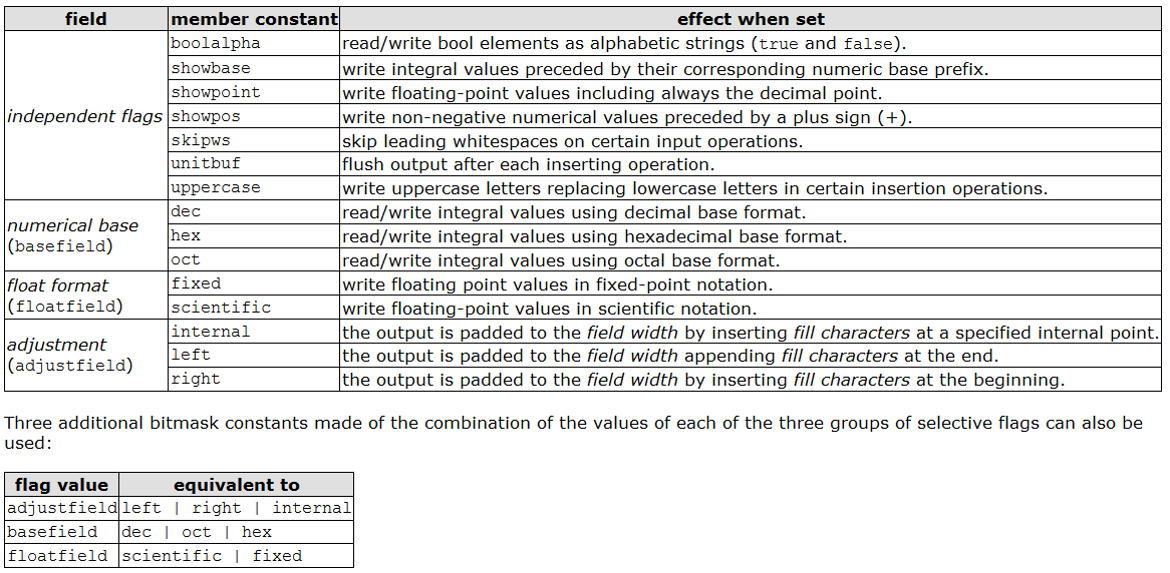
\includegraphics[width=1.0\textwidth]{figure/chap08/05fomatflag}\\
  {\scriptsize
    \url{http://www.cplusplus.com/reference/iostream/ios_base/fmtflags/}}
  \stretchoff
\end{frame}

\begin{frame}[t, fragile]{输出流}{输出流与格式控制}%
  \begin{itemize}
  \item 状态字设置函数   
  \end{itemize}
  \begin{center}
    \scriptsize
    \begin{tabular}{|l|p{3.5cm}|}
      \hline
      函数 & 功能\\
      \hline
      \cppinttscr{long flags( long lFlags );} & 用参数lFlags更新标志字\\
      \cppinttscr{long flags() const;} & 返回标志字\\
      \hline
      \cppinttscr{long setf( long lFlags );} & 设置lFlags指定的标志位\\
      \cppinttscr{long setf( long lFlags, long lMask );} & 将lMask指定的位清0,然后设置lFlags指定位\\
      \hline
      \cppinttscr{long unsetf( long lFlags );} & 将lMask指定的标志位清0\\
      \hline
    \end{tabular}
  \end{center}
\end{frame}

\begin{frame}[t, fragile]{输出流}{输出流与格式控制}%
  \begin{itemize}
  \item 输出流常用函数(ostream)
  \end{itemize}
  \begin{center}
    \begin{tikzpicture}[font=\tiny, show background grid]
      \tikzset{coord/.style={coordinate}}

      \umlnote[scale=0.6, text width=0.6\textwidth] (code1) at (0, 0)
      {
        \cppfilenobg{codes/chap08/testIOFlag/main.cpp}
      };

      \path let \p1=(code1) in
      coordinate (org) at (\x1, \y1)
      coordinate (ovBL1) at ($(org) + (-2.20, -1.96)$)
      coordinate (ovUR1) at ($(ovBL1) + (0.45, 0.0)$)
      coordinate (ovBL2) at ($(ovBL1) + (0.0, -0.15)$)
      coordinate (ovUR2) at ($(ovBL2) + (0.65, 0.0)$)
      ;

      \draw[red, thick] (ovBL1) -- (ovUR1);
      \draw[blue, thick] (ovBL2) -- (ovUR2);
      
      \umlnote[scale=0.6, text width=0.66\textwidth] (code2) at ($(code1.south) + (2.0, 0.2)$)
      {
        \begin{tabular}{|c|c|c|c|c|c|c|c|c|c|c|c|c|c|c|c|}
          % \\
          \multicolumn{16}{c}{}\\
          \hline
        0 & 0 & 0 & 1 & 0 & 0 & 0 & 0 & 0 & 0 & 0 & 0 & \textcolor{red}{0} & 0 & \textcolor{red}{1} & 0\\\hline
        0 & 0 & 0 & 1 & 0 & 0 & 0 & 0 & 0 & 0 & 0 & 0 & \textcolor{red}{1} & 0 & \textcolor{red}{0} & 0\\
        \hline
        \end{tabular}
      };

      \umlnote[scale=0.6, text width=0.22\textwidth] (code3) at ($(code1.east) + (-1.0, -1.0)$)
      {
        \begin{tabular}{|c|l|r|}
          \hline
          dec & 2 & \textcolor{red}{10}\\\hline
          hec & 8 & \textcolor{red}{100}\\\hline
          oct & 40 & \textcolor{red}{1000000}\\
        \hline
        \end{tabular}
      };

      \path let \p1=(code2) in
      coordinate (org) at (\x1, \y1)
      coordinate (ovBL3) at ($(org) + (-2.65, -0.00)$)
      coordinate (ovBL4) at ($(ovBL3) + (0.0, -0.15)$)
      ;

      \draw[-{Stealth[scale=1.0]}, red, thick] (ovBL1) to[out=180, in=180] (ovBL3);
      \draw[-{Stealth[scale=1.0]}, blue, thick] (ovBL2) to[out=180, in=180] (ovBL4);

      
    \end{tikzpicture}
  \end{center}
\end{frame}

\begin{frame}[ t, fragile]{输出流}{输出流与格式控制}%
  \stretchon
  \begin{itemize}
  \item 格式控制成员函数
    \begin{itemize}
    \item 设置域宽: \cppinttfts{int width(int nw);}
    \item 填充: \cppinttfts{fill(char c);}
    \item 设置浮点数精度: \cppinttfts{int precision(int n);}
    \item 设置格式: \cppinttfts{long flags(long lFlags);}
    \end{itemize}
  \end{itemize}
  \stretchoff
\end{frame}

\begin{frame}[t, fragile]{输出流}{输出流与格式控制}%
  \stretchon
  \begin{itemize}
  \item 格式操纵符:简化I/O格式化操作 (iomanip)
    \begin{itemize}
    \item 进制(dec、oct、hex和setbase())
    \item 对齐
    \item 浮点数显示
    \item 设置当前域宽(setw)
    \item 填充(setfill)
    \item 设置精度(setprecision)
    \item $\cdots$
    \end{itemize}
  \end{itemize}
  \stretchoff
\end{frame}

\begin{frame}[t, fragile]{输出流}{输出流与格式控制}%
  \begin{itemize}
  \item 格式操纵符:简化I/O格式化操作
  \end{itemize}
  \begin{center}
    \begin{tikzpicture}[font=\tiny, show background grid]
      \tikzset{coord/.style={coordinate}}

      \umlnote[scale=1.2, text width=0.7\textwidth] (code1) at (0, 0)
      {
        \cppfilenobg{codes/chap08/testFormat/main-main.cpp}
      };

      \path let \p1=(code1) in
      coordinate (org) at (\x1, \y1)
      coordinate (ovBL1) at ($(org) + (-5.15, -0.25)$)
      coordinate (ovUR1) at ($(ovBL1) + (1.46, 0.3)$)
      ;

      \draw[red,thick,fill=green!25, fill opacity=0.35] (ovBL1) rectangle (ovUR1);
    \end{tikzpicture}
  \end{center}
\end{frame}

\begin{frame}[t, fragile]{输出流}{输出流与格式控制}%
  \begin{itemize}
  \item 格式控制成员函数
  \end{itemize}
  \begin{center}
    \begin{tikzpicture}[font=\tiny, show background grid]
      \tikzset{coord/.style={coordinate}}

      \umlnote[scale=0.9, text width=0.7\textwidth] (code1) at (0, 0)
      {
        \cppfilenobg{codes/chap08/testFormat02/main.cpp}
      };

      % \path let \p1=(code1) in
      % coordinate (org) at (\x1, \y1)
      % coordinate (ovBL1) at ($(org) + (-3.82, -0.26)$)
      % coordinate (ovUR1) at ($(ovBL1) + (1.55, 0.3)$)
      % ;

      % \draw[red,thick,fill=green!25, fill opacity=0.55] (ovBL1) rectangle (ovUR1);
    \end{tikzpicture}
  \end{center}
\end{frame}
%%%%%%%%%%%%%%%%%%%%%%%%%%%%%%%%%%%%%%%%%%%%%%%%%%%%%%%%%%%%%%%%%%%%%%%%%%%%%%%

\section[输入流]{输入流}\label{sec:chap08-sec03}
%%%%%%%%%%%%%%%%%%%%%%%%%%%%%%%%%%%%%%%%%%%%%%%%%%%%%%%%%%%%%%%%%%%%%%%%%%%%%%%
\begin{frame}[t, fragile]{输入流}{输入流常用函数}%
  
  \begin{itemize}
  \item 输入流常用函数(istream)
  \end{itemize}
  \begin{center}
    \begin{tabular}[h]{|l|p{4.5cm}|}
      \hline
      \cppinline{read} & 无格式输入指定字节数 \\ \hline
      \cppinline{get} & 从流中提取字符,包括空格 \\ \hline
      \cppinline{getline} & 从流中提取一行字符 \\ \hline
      \cppinline{seekg} & 移动输入流指针 \\ \hline
      \cppinline{operstor>>} & 输入运算符 \\ \hline
    \end{tabular}
  \end{center}
\end{frame}

\begin{frame}[t, fragile]{输入流}{输入流常用函数}%
  \begin{itemize}
  \item 输入流常用函数get()
  \end{itemize}
  \begin{center}
    \begin{tikzpicture}[font=\tiny, show background grid]
      \tikzset{coord/.style={coordinate}}

      \umlnote[scale=1.0, text width=0.7\textwidth] (code1) at (0, 0)
      {
        \cppfilenobg{codes/chap08/testGet/main.cpp}
      };

      \path let \p1=(code1) in
      coordinate (org) at (\x1, \y1)
      coordinate (ovBL1) at ($(org) + (-3.10, -0.08)$)
      coordinate (ovUR1) at ($(ovBL1) + (1.06, 0.3)$)
      coordinate (ovBL2) at ($(ovBL1) + (-1.24, -1.56)$)
      coordinate (ovUR2) at ($(ovBL2) + (1.75, 0.3)$)
      ;

      \draw[red,thick,fill=green!25, fill opacity=0.55] (ovBL1) rectangle (ovUR1);
      \draw[red,thick,fill=green!25, fill opacity=0.55] (ovBL2) rectangle (ovUR2);
    \end{tikzpicture}
  \end{center}
\end{frame}

\begin{frame}[t, fragile]{输入流}{输入流常用函数}%
  \begin{itemize}
  \item 输入流常用函数getline
  \end{itemize}
  \begin{center}
    \begin{tikzpicture}[font=\tiny, show background grid]
      \tikzset{coord/.style={coordinate}}

      \umlnote[scale=1.0, text width=0.7\textwidth] (code1) at (0, 0)
      {
        \cppfilenobg{codes/chap08/testGetline/main.cpp}
      };

      \path let \p1=(code1) in
      coordinate (org) at (\x1, \y1)
      coordinate (ovBL1) at ($(org) + (-3.42, -0.71)$)
      coordinate (ovUR1) at ($(ovBL1) + (2.77, 0.3)$)
      ;

      \draw[red,thick,fill=green!25, fill opacity=0.55] (ovBL1) rectangle (ovUR1);
    \end{tikzpicture}
  \end{center}
\end{frame}

\begin{frame}[t, fragile]{输入流}{输入流常用函数}%
  \begin{itemize}
  \item 输入流常用函数getline
  \end{itemize}
  \begin{center}
    \begin{tikzpicture}[font=\tiny, show background grid]
      \tikzset{coord/.style={coordinate}}

      \umlnote[scale=1.0, text width=0.7\textwidth] (code1) at (0, 0)
      {
        \cppfilenobg{codes/chap08/testGetline02/main.cpp}
      };

      \path let \p1=(code1) in
      coordinate (org) at (\x1, \y1)
      coordinate (ovBL1) at ($(org) + (-3.42, -0.71)$)
      coordinate (ovUR1) at ($(ovBL1) + (3.22, 0.3)$)
      ;

      \draw[red,thick,fill=green!25, fill opacity=0.55] (ovBL1) rectangle (ovUR1);
    \end{tikzpicture}
  \end{center}
\end{frame}


\section[文本文件]{文本文件的输入输出}\label{sec:chap08-sec04}
%%%%%%%%%%%%%%%%%%%%%%%%%%%%%%%%%%%%%%%%%%%%%%%%%%%%%%%%%%%%%%%%%%%%%%%%%%%%%%%
\begin{frame}[t, fragile]{文本文件}{简介}%
  \stretchon
  \begin{itemize}
  \item 文件的创建
    \begin{itemize}
    \item 方法1
      \begin{itemize}
      \item 使用ifstream、ofstream或fstream类建立文件流对象(无参构造
        函数)
      \item 调用成员函数open建立文件
      \end{itemize}
    \item 方法2
      \begin{itemize}
      \item 使用ifstream、ofstream或fstream类建立文件流对象(调用带参数构造函数)
      \end{itemize}
    \end{itemize}
  \end{itemize}
  \stretchoff
\end{frame}

\begin{frame}[t, fragile]{文本文件}{创建文件}%
  \begin{itemize}
  \item 文件的创建    
  \end{itemize}
  \begin{center}
    \begin{tikzpicture}[font=\tiny, show background grid]
      \tikzset{coord/.style={coordinate}}

      \umlnote[scale=1.0, text width=0.6\textwidth] (code1) at (0, 0)
      {
        \begin{cppttnobg}
fstream file;
file.open("d:\\data\\exe1.txt", ios::out);
file.close();
        \end{cppttnobg}
      };

      \umlnote[scale=1.0, text width=0.6\textwidth] (code2) at (0, -2.5)
      {
        \begin{cppttnobg}
fstream file("d:\\data\\exe1.txt", ios::out);
file.close();
        \end{cppttnobg}
      };

      \draw[implies-implies,double equal sign distance] (code1.south) -- (code2.north);
    \end{tikzpicture}
  \end{center}
\end{frame}

\begin{frame}[t, fragile]{文本文件}{创建文件}%
  \begin{itemize}
  \item 文件的创建    
  \end{itemize}
  \begin{center}
    \begin{tikzpicture}[font=\tiny, show background grid]
      \tikzset{coord/.style={coordinate}}

      \umlnote[scale=1.0, text width=0.6\textwidth] (code1) at (0, 0)
      {
        \begin{cppttnobg}
fstream file;
file.open("d:\\data\\exe1.txt", ios::out);
file.close();
        \end{cppttnobg}
      };

      \umlnote[scale=1.0, text width=0.6\textwidth] (code2) at (0, -2.5)
      {
        \begin{cppttnobg}
ofstream file;
file.open("d:\\data\\exe1.txt");
file.close();
        \end{cppttnobg}
      };

      \draw[implies-implies,double equal sign distance] (code1.south) -- (code2.north);
    \end{tikzpicture}
  \end{center}
\end{frame}

\begin{frame}[t, fragile]{文本文件}{创建文件}%
  \begin{itemize}
  \item 文件的创建    
  \end{itemize}
  \begin{center}
    \begin{tikzpicture}[font=\tiny, show background grid]
      \tikzset{coord/.style={coordinate}}

      \umlnote[scale=1.0, text width=0.6\textwidth] (code1) at (0, 0)
      {
        \begin{cppttnobg}
fstream file;
file.open("d:\\data\\exe1.txt", ios::in);
file.close();
        \end{cppttnobg}
      };

      \umlnote[scale=1.0, text width=0.6\textwidth] (code2) at (0, -2.5)
      {
        \begin{cppttnobg}
ifstream file;
file.open("d:\\data\\exe1.txt");
file.close();
        \end{cppttnobg}
      };

      \draw[implies-implies,double equal sign distance] (code1.south) -- (code2.north);
    \end{tikzpicture}
  \end{center}
\end{frame}

\begin{frame}[t, fragile]{文本文件}{写操作}%
  \begin{itemize}
  \item 文本文件的写操作
  \end{itemize}
  \begin{center}
    \begin{tikzpicture}[font=\tiny, show background grid]
      \tikzset{coord/.style={coordinate}}

      \umlnote[scale=0.9, text width=0.6\textwidth] (code1) at (0, 0)
      {
        \cppfilenobg{codes/chap08/testTXTWrite/main.cpp}
      };
    \end{tikzpicture}
  \end{center}
\end{frame}

\begin{frame}[t, fragile]{文本文件}{读操作}%
  \begin{itemize}
  \item 文本文件的读操作
  \end{itemize}
  \begin{center}
    \begin{tikzpicture}[font=\tiny, show background grid]
      \tikzset{coord/.style={coordinate}}

      \umlnote[scale=0.9, text width=0.7\textwidth] (code1) at (0, 0)
      {
        \cppfilenobg{codes/chap08/testTXTRead/main.cpp}
      };
    \end{tikzpicture}
  \end{center}
\end{frame}

\begin{frame}[t, fragile]{文本文件}{合并操作}%
  \begin{itemize}
  \item 文件合并排序操作
    \begin{itemize}
    \item 高考成绩
    \item 姓名、准考证号、所考大学、总成绩
    \item 准考证号是关键字
    \item 有\alert{重复记录}
    \item \alert{合并,去掉重复记录,并按准考证号升序排列}
    \end{itemize}
  \end{itemize}
  \begin{center}
    \begin{tikzpicture}[font=\tiny, show background grid]
      \tikzset{coord/.style={coordinate}}

      \umlnote[scale=0.9, text width=0.8\textwidth] (code1) at (0, 0)
      {
        \cppfilenobg{codes/chap08/testFileMerginSort/01-structdef.cpp}
      };
    \end{tikzpicture}
  \end{center}
\end{frame}

\begin{frame}[t, fragile]{文本文件}{合并操作}%
  \begin{itemize}
  \item 文件合并排序操作    
  \end{itemize}
  \begin{center}
    \begin{tikzpicture}[font=\tiny, show background grid]
      \tikzset{coord/.style={coordinate}}

      \umlnote[scale=1.0, text width=0.8\textwidth] (code1) at (0, 0)
      {
        \cppfilenobg{codes/chap08/testFileMerginSort/02-readfilefun.cpp}
      };
    \end{tikzpicture}
  \end{center}
\end{frame}

\begin{frame}[t, fragile]{文本文件}{合并操作}%
  \begin{itemize}
  \item 文件合并排序操作    
  \end{itemize}
  \begin{center}
    \begin{tikzpicture}[font=\tiny, show background grid]
      \tikzset{coord/.style={coordinate}}

      \umlnote[scale=1.0, text width=0.8\textwidth] (code1) at (0, 0)
      {
        \cppfilenobg{codes/chap08/testFileMerginSort/03-printfilefun.cpp}
      };
    \end{tikzpicture}
  \end{center}
\end{frame}

\begin{frame}[t, fragile]{文本文件}{合并操作}%
  \begin{itemize}
  \item 文件合并排序操作    
  \end{itemize}
  \begin{center}
    \begin{tikzpicture}[font=\tiny, show background grid]
      \tikzset{coord/.style={coordinate}}

      \umlnote[scale=0.9, text width=0.8\textwidth] (code1) at (0, 0)
      {
        \cppfilenobg{codes/chap08/testFileMerginSort/04-mainfun.cpp}
      };
    \end{tikzpicture}
  \end{center}
\end{frame}
%%%%%%%%%%%%%%%%%%%%%%%%%%%%%%%%%%%%%%%%%%%%%%%%%%%%%%%%%%%%%%%%%%%%%%%%%%%%%%%

\section[二进制文件]{二进制文件的输入输出}\label{sec:chap08-sec05}
%%%%%%%%%%%%%%%%%%%%%%%%%%%%%%%%%%%%%%%%%%%%%%%%%%%%%%%%%%%%%%%%%%%%%%%%%%%%%%%
\begin{frame}[t, fragile]{二进制文件}{输出}%
  \begin{itemize}
  \item 二进制文件的输出
  \end{itemize}
  \begin{center}
    \begin{tikzpicture}[font=\tiny, show background grid]
      \tikzset{coord/.style={coordinate}}

      \umlnote[scale=0.8, text width=0.8\textwidth] (code1) at (0, 0)
      {
        \cppfilenobg{codes/chap08/testbiFileWrite/main.cpp}
      };

      \umlnote[scale=0.75, text width=0.35\textwidth] (code2) at (1.5, -0.5)
      {
        \begin{cpptt}
ostream& write(const char* s , streamsize n);
        \end{cpptt}
      };

      \path let \p1=(code1) in
      coordinate (org) at (\x1, \y1)
      coordinate (ovBL1) at ($(org) + (-0.95, 0.35)$)
      coordinate (ovUR1) at ($(ovBL1) + (1.02, 0.3)$)
      coordinate (ovBL2) at ($(ovBL1) + (-2.82, -2.27)$)
      coordinate (ovUR2) at ($(ovBL2) + (3.75, 0.47)$)
      ;

      \draw[red,thick,fill=green!25, fill opacity=0.55] (ovBL1) rectangle (ovUR1);
      \draw[blue,thick,fill=blue!25, fill opacity=0.35] (ovBL2) rectangle (ovUR2);
    \end{tikzpicture}
  \end{center}
\end{frame}

\begin{frame}[t, fragile]{二进制文件}{输入}%
  \begin{itemize}
  \item 二进制文件的输入
  \end{itemize}
  \begin{center}
    \begin{tikzpicture}[font=\tiny, show background grid]
      \tikzset{coord/.style={coordinate}}

      \umlnote[scale=0.8, text width=0.8\textwidth] (code1) at (0, 0)
      {
        \cppfilenobg{codes/chap08/testBiFileRead/main.cpp}
      };

      \umlnote[scale=0.9, text width=0.35\textwidth] (code2) at (1.5, -0.5)
      {
        \begin{cpptt}
istream& read(char* s, streamsize n);
        \end{cpptt}
      };

      \path let \p1=(code1) in
      coordinate (org) at (\x1, \y1)
      coordinate (ovBL1) at ($(org) + (-1.05, 0.35)$)
      coordinate (ovUR1) at ($(ovBL1) + (1.02, 0.3)$)
      coordinate (ovBL2) at ($(ovBL1) + (-2.75, -2.07)$)
      coordinate (ovUR2) at ($(ovBL2) + (3.85, 0.47)$)
      ;

      \draw[red,thick,fill=green!25, fill opacity=0.55] (ovBL1) rectangle (ovUR1);
      \draw[blue,thick,fill=blue!25, fill opacity=0.35] (ovBL2) rectangle (ovUR2);
    \end{tikzpicture}
  \end{center}
\end{frame}

\begin{frame}[t, fragile]{二进制文件}{输入}%
  \begin{itemize}
  \item 二进制文件的输入
  \end{itemize}
  \begin{center}
    \begin{tikzpicture}[font=\tiny, show background grid]
      \tikzset{coord/.style={coordinate}}

      \umlnote[scale=0.9, text width=0.6\textwidth] (fig1) at (0, 0)
      {
        \includegraphics[width=0.45\textwidth]{codes/chap08/testImageReadWrite/Lighthouse.bmp}
        \qquad
        \includegraphics[width=0.45\textwidth]{codes/chap08/testImageReadWrite/Penguins.bmp}
      };

      \umlnote[scale=0.9, text width=0.3\textwidth] (fig2) at (0, -3.5)
      {
        \includegraphics[width=0.9\textwidth]{codes/chap08/testImageReadWrite/Result.bmp}
      };  
    \end{tikzpicture}
  \end{center}
\end{frame}

\begin{frame}[t, fragile]{二进制文件}{输入}%
  \begin{itemize}
  \item 二进制文件的输入
  \end{itemize}
  \begin{center}
    \begin{tikzpicture}[font=\tiny, show background grid]
      \tikzset{coord/.style={coordinate}}

      \umlnote[scale=0.9, text width=0.9\textwidth] (code1) at (0, 0)
      {
        \cppfilenobg{codes/chap08/testImageReadWrite/01-strucdef.cpp}
      };     
    \end{tikzpicture}
  \end{center}
\end{frame}

\begin{frame}[t, fragile]{二进制文件}{输入}%
  \begin{itemize}
  \item 二进制文件的输入
  \end{itemize}
  \begin{center}
    \begin{tikzpicture}[font=\tiny, show background grid]
      \tikzset{coord/.style={coordinate}}

      \umlnote[scale=0.8, text width=0.9\textwidth] (code1) at (0, 0)
      {
        \cppfilenobg{codes/chap08/testImageReadWrite/02-mainfun-01.cpp}
      };     
    \end{tikzpicture}
  \end{center}
\end{frame}

\begin{frame}[t, fragile]{二进制文件}{输入}%
  \begin{itemize}
  \item 二进制文件的输入
  \end{itemize}
  \begin{center}
    \begin{tikzpicture}[font=\tiny, show background grid]
      \tikzset{coord/.style={coordinate}}

      \umlnote[scale=0.9, text width=0.9\textwidth] (code1) at (0, 0)
      {
        \cppfilenobg{codes/chap08/testImageReadWrite/03-mainfun-02.cpp}
      };     
    \end{tikzpicture}
  \end{center}
\end{frame}


%%%%%%%%%%%%%%%%%%%%%%%%%%%%%%%%%%%%%%%%%%%%%%%%%%%%%%%%%%%%%%%%%%%%%%%%%%%%%%%
% 附件页
\section[附件下载]{本讲示例代码及附件下载} 
\begin{frame}{附件}{本讲附件}
  % 此处的[ucfilespec=...]必须指定为pdf否则Windows下无法下载
  %\vspace{-4ex}
  \textattachfile[ucfilespec=ex-src08.pdf]{ex-src08.zip}{附件:右键单击该
    链接,选择\qtmark{\alert{保存附件}}下载,\alert{将后缀名改为\qtmark{.zip}解压}
      \footnote[frame]{请\alert{退出全屏模式}后点击该链接。}
      \footnote[frame]{以Adobe Acrobat Reader为例。}
      。}%\\

  \vspace{-1ex}
  \begin{center}
    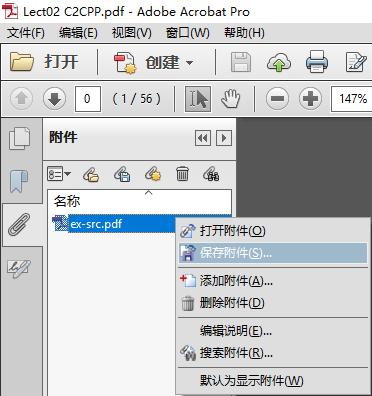
\includegraphics[height=0.35\textheight]{pdfattatchdownload01}\quad
    %或 \quad%
    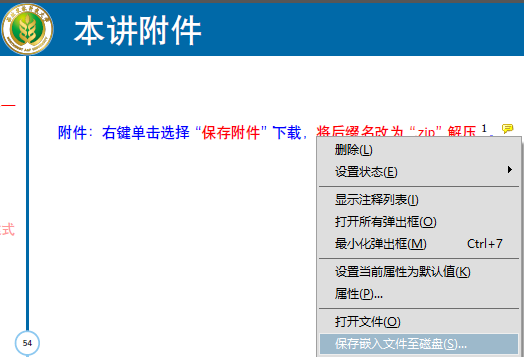
\includegraphics[height=0.35\textheight]{pdfattatchdownload02}\\[2ex]%
    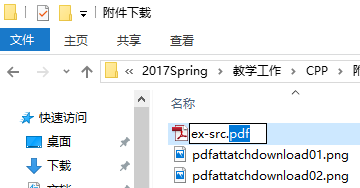
\includegraphics[height=0.255\textheight]{pdfattatchdownload03}\quad
    %$\Rightarrow$ \quad%
    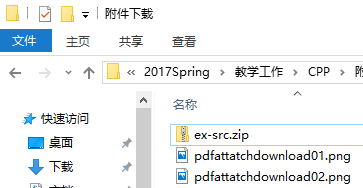
\includegraphics[height=0.255\textheight]{pdfattatchdownload04}%
  \end{center}   
\end{frame}



% \tiny
% \scriptsize
% \footnotesize
% \small
% \normalsize
% \large
% \Large
% \LARGE
% \huge
% \Huge


%%% Local Variables: 
%%% mode: latex
%%% TeX-master: "../main.tex"
%%% End: 
